\chapter{A memória que aprende}\label{cap:memoria}

O capítulo da partilha terminou numa frase que pede conta. A escala é o ingrediente que precisa ser
atualizado sempre, e atualizar é trocar passado por presente. Quanto do passado se pode apagar antes
que o sistema deixe de aprender?

\section{A janela de um ano, num mundo que muda}

O primeiro capítulo deste livro fixou uma janela de um ano para o corte, e ela funciona lá. Levada
para a escala de um mundo que dobra de uma vez, a mesma janela erra por \numEsquecimentoJanelaDuzentosECinquenta{}
no ano seguinte à mudança. É um erro de um quarto, e ele não se anuncia: no mundo que não muda, a
mesma janela erra por \numEsquecimentoPisoJanelaDuzentosECinquenta{}, que é pouco. Quem só olha o mundo
parado conclui que a janela está calibrada.

O defeito tem nome: uma janela carrega os dias velhos com o mesmo peso dos novos, e no dia em que
eles completam o tamanho da janela, todos caem de uma vez. É esse degrau de saída que faz o erro
grande justamente quando o mundo acabou de mudar.

\section{Esquecer tem taxa}

A outra maneira de estimar o nível não tem tamanho de janela; tem \textbf{taxa}.

% aterramento: esquecimento
% aterramento: lambda
\begin{definicao}[esquecimento com taxa]\label{def:esquecimento}
A estimativa de hoje é uma mistura da estimativa de ontem com a observação de hoje, com peso
$\lambda$ para hoje:
\[
\hat m_t = (1-\lambda)\,\hat m_{t-1} + \lambda\, x_t .
\]
A \emph{memória efetiva} dessa taxa é $1/\lambda$ dias \cite{box2008time}. A \emph{janela deslizante} de $n$ dias é a
média dos últimos $n$ dias, e é a forma que o resto do livro usa.
\end{definicao}

Lida com números: com $\lambda$ de um vigésimo primeiro por dia a memória efetiva é de
\numEsquecimentoMelhorMemoria{} dias, que é a memória que este capítulo vai medir como a melhor da
varredura, e com $\lambda$ de um décimo ela é de dez dias, de modo que a estimativa segue o dia de
hoje de perto.

Com $\lambda$ perto de zero a estimativa quase não se move, e o sistema lembra de um passado muito
longo. Com $\lambda$ igual a um a estimativa é o dia de hoje, e não há estimativa nenhuma. As duas
pontas são conhecidas; o que se quer saber é onde fica o meio \cite{dahlhaus1998optimal}.

% aterramento: epsilon
Quando a pergunta é quanto tempo a estimativa leva para voltar a valer, é preciso dizer o que é
voltar a valer: $\epsilon$ é o erro que ainda se aceita, e a proposição o mede em fração do
\emph{degrau}. A medição declara a tolerância na unidade do \emph{nível} novo --- os
\numEsquecimentoTolerancia{} do nível ---, e as duas unidades se convertem: no mundo que dobra de
uma vez, a mesma tolerância vale o dobro em fração do degrau. A resposta da proposição é em quantos
dias a estimativa cruza a fronteira.
% aterramento: meia-vida
\begin{proposicao}[a meia-vida e a janela]\label{prop:meia-vida}
Num mundo cujo nível dobra de uma vez no instante $t_0$, o desvio da estimativa com taxa $\lambda$
em relação ao nível novo é, em $t_0 + t$,
\[
\hat m_{t_0+t} - L_2 \;=\; (1-\lambda)^{t+1}\big(\hat m_{t_0-1} - L_2\big),
\]
de modo que cruzar até uma tolerância $\epsilon$ do degrau leva
$\log \epsilon / \log(1-\lambda)$ dias contados do último dia do nível antigo --- um dia menos
quando se contam os dias desde a mudança. Na janela deslizante de $n$ dias, o mesmo desvio cai
linearmente e chega a zero exatamente $n$ dias depois da mudança.
\end{proposicao}

\begin{proof}
Do dia da mudança em diante o nível é $L_2$, de modo que o desvio $d_t = \hat m_t - L_2$ obedece
$d_t = (1-\lambda) d_{t-1}$ --- e já no próprio dia da mudança, porque o estimador carrega o dia
anterior. A recursão é geométrica, e contando a partir do último dia do nível antigo ela dá a forma
fechada acima; dividindo $\log\epsilon$ por $\log(1-\lambda)$ chega-se aos dias daquele dia. Para a janela, a média dos últimos $n$ dias
é $L_2$ menos a fração dos seus dias que ainda são anteriores a $t_0$ vezes o tamanho do degrau; essa
fração cai de um a zero em $n$ dias, e depois disso nenhum dia velho entra na média.
\end{proof}

A proposição diz o que a medição vai confirmar: a janela é exata depois de $n$ dias, e a taxa nunca
é exata, porque sempre guarda um resto de tudo o que viu.

\section{A medição}

O mundo é o de sempre: uma oscilação que multiplica por \numEsquecimentoFator{} de uma vez, no dia
\numEsquecimentoQuando{} de \numEsquecimentoDiasDeSerie{} dias, avaliada em \numEsquecimentoSementes{} mundos sorteados. O erro é a distância relativa média
entre a estimativa e a verdade declarada, dia a dia.

\begin{table}[htbp]
  \centering
  \small
  \begin{tabular}{rrrrr}
    \hline
    memória & erro da & erro da & piso da & dias previstos \\
    (dias) & mistura & janela & mistura & até \numEsquecimentoTolerancia{} do nível \\
    \hline
    mil & \numEsquecimentoErroMil & \numEsquecimentoJanelaMil & \numEsquecimentoPisoMil & \numEsquecimentoDiasMil \\
    duzentos e cinquenta & \numEsquecimentoErroDuzentosECinquenta & \numEsquecimentoJanelaDuzentosECinquenta & \numEsquecimentoPisoDuzentosECinquenta & \numEsquecimentoDiasDuzentosECinquenta \\
    cinquenta & \numEsquecimentoErroCinquenta & \numEsquecimentoJanelaCinquenta & \numEsquecimentoPisoCinquenta & \numEsquecimentoDiasCinquenta \\
    vinte e um & \numEsquecimentoErroVinteEUm & \numEsquecimentoJanelaVinteEUm & \numEsquecimentoPisoVinteEUm & \numEsquecimentoDiasVinteEUm \\
    dez & \numEsquecimentoErroDez & \numEsquecimentoJanelaDez & \numEsquecimentoPisoDez & \numEsquecimentoDiasDez \\
    cinco & \numEsquecimentoErroCinco & \numEsquecimentoJanelaCinco & \numEsquecimentoPisoCinco & \numEsquecimentoDiasCinco \\
    dois & \numEsquecimentoErroDois & \numEsquecimentoJanelaDois & \numEsquecimentoPisoDois & \numEsquecimentoDiasDois \\
    um & \numEsquecimentoErroUm & \numEsquecimentoJanelaUm & \numEsquecimentoPisoUm & \numEsquecimentoDiasUm \\
    \hline
  \end{tabular}
  \caption{O erro nos \numEsquecimentoHorizonte{} dias seguintes ao degrau, o erro no mundo que não
    muda e os dias que a \cref{prop:meia-vida} prevê para chegar a \numEsquecimentoTolerancia{} do
    nível novo --- que, num mundo que dobra de uma vez, é \numEsquecimentoToleranciaDegrau{} do
    degrau. A memória é a
    memória efetiva: o inverso da taxa, para a mistura, e o número de dias, para a janela.}
  \label{tab:esquecimento}
\end{table}

\begin{figure}[htbp]
  \centering
  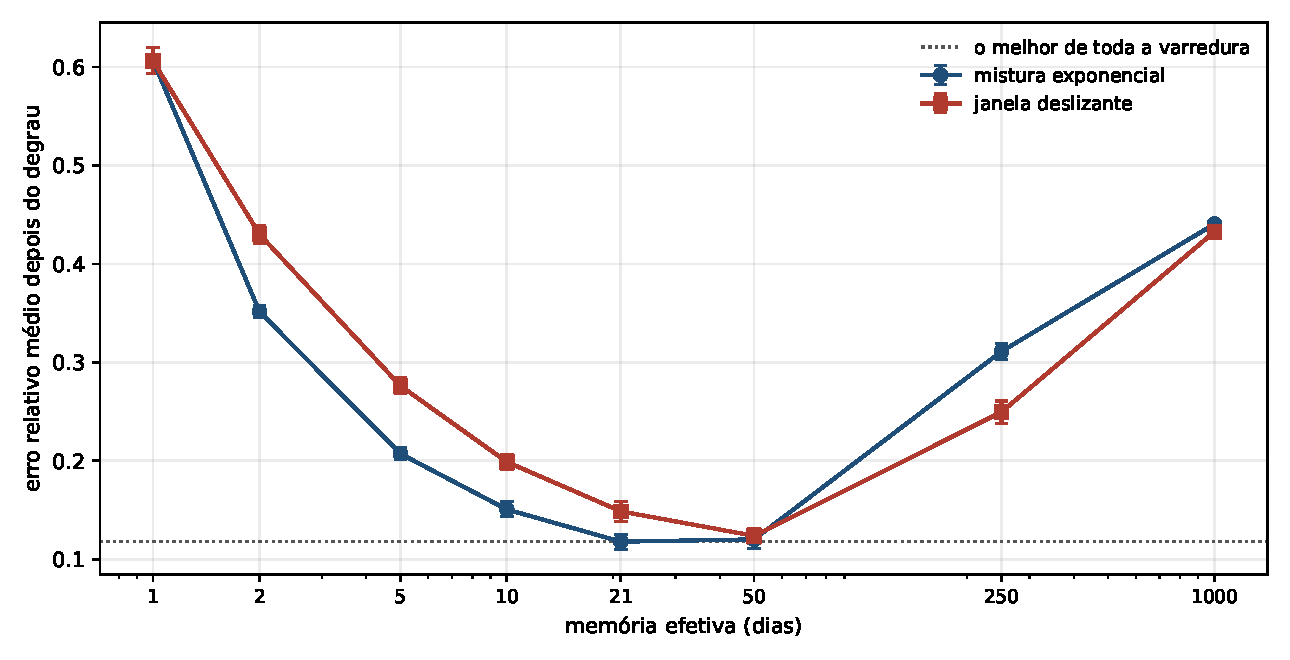
\includegraphics[width=\linewidth]{figuras/E12_esquecimento_1.pdf}
  \caption{O erro depois do degrau contra a memória efetiva, nas duas formas de esquecer. A linha
    pontilhada é o melhor erro de toda a varredura. O eixo da memória é logarítmico: distâncias iguais
    no papel são multiplicações iguais no tempo de memória.}
  \label{fig:esquecer}
\end{figure}

A leitura da tabela tem três partes. A memória de mil dias erra por \numEsquecimentoErroMil{} e a de
um dia por \numEsquecimentoErroUm{}: as duas pontas são ruins, e por motivos opostos. A memória de
\numEsquecimentoMelhorMemoria{} dias é a melhor, com \numEsquecimentoErroVinteEUm{} e dispersão de
\numEsquecimentoMelhorDispersao{} --- e o piso de ruído dela é \numEsquecimentoPisoNaMelhor{}, de modo
que no melhor desenho quase todo o erro que sobra é ruído, e não atraso. A pergunta "quanto do passado se pode apagar" tem, então, uma resposta em duas partes:
apaga-se até a memória de vinte e um dias, e o que sobra depois disso já não é passado, é o tamanho
da amostra.

Sobre a referência declarada, a janela: com memória de vinte e um dias ela erra por
\numEsquecimentoJanelaVinteEUm{} contra \numEsquecimentoErroVinteEUm{} da mistura, e o melhor dela
aparece com \numEsquecimentoMelhorJanela{} dias, erro de \numEsquecimentoMelhorJanelaErro{}. A
janela perde para a mistura nas memórias curtas, e a proposição explica: a janela joga fora os dias de
uma vez, e a queda brusca machuca tanto quanto a entrada lenta.

\section{O que cabe prometer}

Falta a conta que decide se um esquecimento \textbf{ainda aprende}, e ela depende do tempo que se tem
para aprender. Com uma tolerância declarada de \numEsquecimentoTolerancia{} do nível novo --- o
mesmo que \numEsquecimentoToleranciaDegrau{} do degrau, porque o mundo aqui dobra de uma vez ---,
varrendo as memórias e os horizontes, dos \numEsquecimentoParesTodos{} pares testados apenas
\numEsquecimentoParesViaveis{} aprendem.

\begin{table}[htbp]
  \centering
  \small
  \begin{tabular}{rrr}
    \hline
    horizonte & melhor erro no & memória que o \\
    (dias) & horizonte & entrega \\
    \hline
    trinta & \numEsquecimentoMelhorNoHorizonteTrinta & \numEsquecimentoMemoriaDoHorizonteTrinta \\
    quarenta e cinco & \numEsquecimentoMelhorNoHorizonteQuarentaECinco & \numEsquecimentoMemoriaDoHorizonteQuarentaECinco \\
    sessenta & \numEsquecimentoMelhorNoHorizonteSessenta & \numEsquecimentoMemoriaDoHorizonteSessenta \\
    noventa & \numEsquecimentoMelhorNoHorizonteNoventa & \numEsquecimentoMemoriaDoHorizonteNoventa \\
    cento e vinte & \numEsquecimentoMelhorNoHorizonteCentoEVinte & \numEsquecimentoMemoriaDoHorizonteCentoEVinte \\
    duzentos e cinquenta & \numEsquecimentoMelhorNoHorizonteDuzentosECinquenta & \numEsquecimentoMemoriaDoHorizonteDuzentosECinquenta \\
    \hline
  \end{tabular}
  \caption{O melhor erro possível em cada horizonte, e a memória que o entrega. O horizonte é o
    tempo disponível depois da mudança para o sistema aprender o nível novo.}
  \label{tab:horizontes}
\end{table}

O horizonte mais curto que aprende é de \numEsquecimentoHorizonteCurto{} dias, com memória de
\numEsquecimentoMemoriaDoCurto{} dias e erro de \numEsquecimentoErroDoCurto. A memória mais longa
que aprende é de \numEsquecimentoMemoriaLonga{} dias, e ela exige \numEsquecimentoHorizonteDaLonga{}
dias de horizonte para isso. Fora dessa janela de combinações, nenhuma das \numEsquecimentoMemorias{}
memórias testadas entrega a tolerância declarada --- nem esquecendo depressa, nem devagar.

\begin{figure}[htbp]
  \centering
  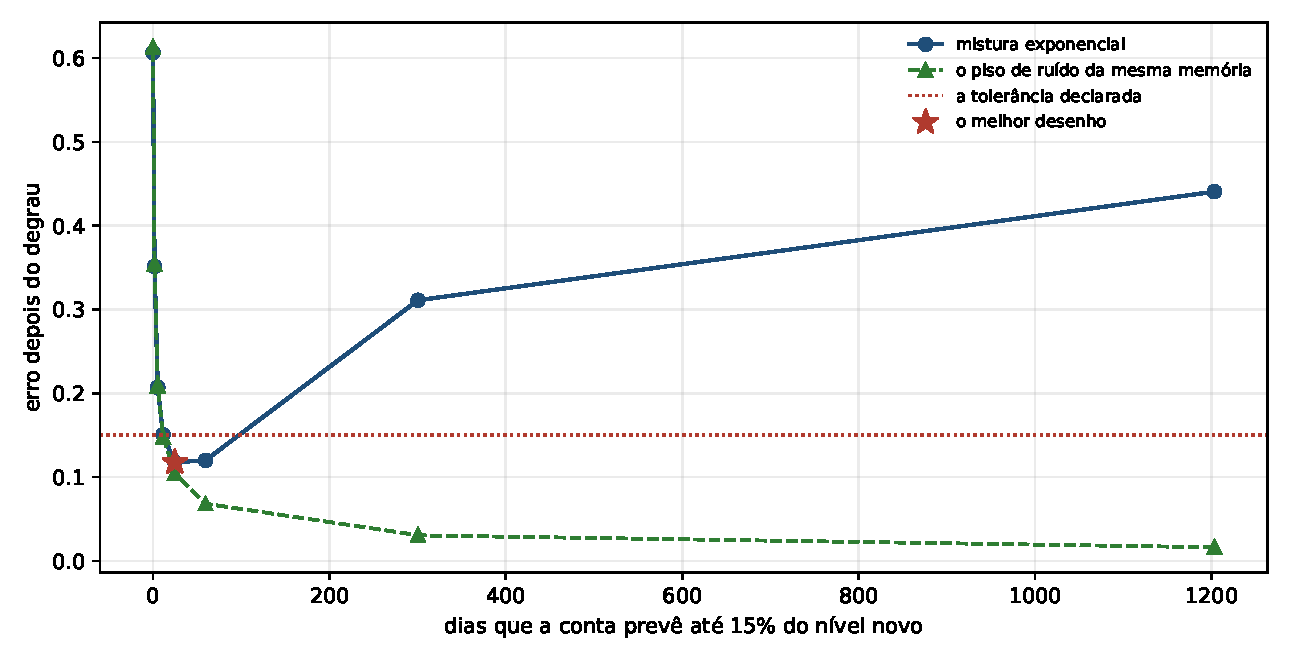
\includegraphics[width=\linewidth]{figuras/E12_esquecimento_2.pdf}
  \caption{O erro depois do degrau contra os dias que a conta do cruzamento prevê até
    \numEsquecimentoTolerancia{} do nível novo. A curva tracejada é o piso de ruído da mesma memória: onde ela alcança a curva de
    cima, o erro deixou de ser atraso e passou a ser tamanho de amostra.}
  \label{fig:prometer}
\end{figure}

A figura mostra o cruzamento que fecha o capítulo. Para memórias curtas as duas curvas andam juntas:
o erro é todo ruído. Para memórias longas elas se separam: o piso cai, o erro total não cai com ele,
e a distância entre as duas é o atraso em relação à mudança. A memória certa é a que minimiza o erro
total, e não a que minimiza a distância entre as duas curvas: as duas quase se tocam nas memórias
curtas, e é lá que o erro ainda é quase todo ruído.

\section{O que fica}

Fica a resposta da travessia, e ela é estreita. O esquecimento mínimo, no sentido da menor memória que entrega a tolerância, é o de vinte e um
dias --- uma taxa de \numEsquecimentoMelhorTaxa{} por
dia ---, e ele exige um horizonte de pelo menos \numEsquecimentoHorizonteCurto{} dias para entregar
\numEsquecimentoTolerancia{} do nível novo, contra os \numEsquecimentoMelhorDias{} dias que a conta
do cruzamento previa para essa mesma memória. Os dois números não se contradizem, porque não medem a
mesma coisa: \numEsquecimentoMelhorDias{} dias é o instante em que o desvio cruza a tolerância, e
\numEsquecimentoHorizonteCurto{} dias é o horizonte em que a \emph{média} do erro fica dentro dela ---
e a média carrega os primeiros dias depois da mudança, quando o desvio ainda é o degrau inteiro. A memória mais longa que ainda entrega a tolerância é a de \numEsquecimentoMemoriaLonga{} dias;
daí para cima, lembrar mais é ficar cego à mudança; quem apaga
mais depressa troca cegueira por ruído, e o erro cresce dos dois lados.

Fica também o que a medição não promete. A melhor combinação de todas erra por
\numEsquecimentoMelhor{}, e é isso que se pode exigir deste estimador neste mundo: pedir menos do que
isso não é um problema de memória, é um problema de amostra. E a janela deslizante, que era a
referência a bater, ficou atrás nas memórias curtas: é ali que ela erra mais, e é ali que o mundo
mudado obriga a escolher.

O fracasso seguinte não fala do nível, e sim do que o esquecimento joga fora junto com os dias velhos.
A memória apaga os dias, e apaga com eles a \textbf{ordem} em que eles vieram --- e é a ordem que diz para
onde o tempo aponta. Nada do que foi construído até aqui distingue uma série do seu próprio filme
rodando ao contrário, e é essa a próxima pergunta.
